%%%%%%%%%%%%%%%%%%%%%%%%%%%%%%%%%%%%%%%%%
% Szablon pracy dyplomowej
% Wydział Informatyki 
% Zachodniopomorski Uniwersytet Technologiczny w Szczecinie
% autor Joanna Kołodziejczyk (jkolodziejczyk@zut.edu.pl)
% Bardzo wczesnym pierwowzorem szablonu był
% The Legrand Orange Book
% Version 2.1 (26/09/2018)
%
% Modifications to LOB assigned by %JK
%%%%%%%%%%%%%%%%%%%%%%%%%%%%%%%%%%%%%%%%%


%----------------------------------------------------------------------------------------
%	CHAPTER 2
%----------------------------------------------------------------------------------------

\chapter{Zebranie materiału uczącego}\label{ch:preparing_data_set}
\chaptermark{Zebranie materiału uczącego} % Tekst, który wyświetli się w nagłówku strony,  jeżeli jest za długi tytuł rozdziału

Niewątpliwą przyczyną rozwoju dziedziny uczenia maszynowego na przestrzeni ostatnich lat jest wzrost wydajności komputerów będących w stanie zbierać i przetwarzać ogromne ilości danych.
Uczenie maszynowe jest obszarem sztucznej inteligencji poświęconej algorytmom, które poprawiają się automatycznie poprzez doświadczenie \cite{Mitchell97}.
Tworząc system automatycznego rozpoznawania tablic rejestracyjnych niezbędne jest przygotowanie odpowiedniego zbioru danych.
Jedną z kluczowych kwestii przed rozpoczęciem kolekcjonowania informacji, jest ustalenie wielkość zbioru.
Najbardziej powszechnym stosowanym podejściem jest zasada 10 razy.
W tym kontekście oznacza ona, że aby ilość danych była wystarczająca, zbiór danych wejściowych powinien być 10 razy większy od liczby parametrów w opracowywanym modelu.
Dla modelu o 1000 parametrach, zbiór powinien zawierać 10 tysięcy próbek.
Zwykle jest to jeden z bardziej czasochłonnych etapów podczas tworzenia modeli uczenia maszynowego.

Do przygotowania danych uczących wykorzystano nagrania z rejestratorów wideo zamontowanych w samochodzie.
Zgromadzony materiał został zarejestrowany za pomocą wielu rejestratorów, stąd rozdzielczość oraz liczba klatek na sekundę różni się pomiędzy plikami wideo.
Pozyskane zdjęcia pochodzą zarówna z przejazdów nocnych jak i za dnia.
Udało się również zebrać materiał ze zróżnicowanymi warunkami atmosferycznymi (tj. jazda w deszczu lub jazda w bezchmurny dzień).
Rozdzielczość obrazu zawierała się w zakresie $1920\times 1080$ do $3840\times 2160$ pikseli.
Liczba klatek na sekundę dla części kamer wynosiła 60 klatek na sekundę, a dla pozostałej części 30 klatek na sekundę.
Algorytm przygotowujący dane uczące potrzebował na wejściu wyekstrahowane cechy z konkretnych obiektów.
Aby to osiągnąć, należało przygotować zdjęcia, na których następnie zaznaczone zostaną obiekty.

W pierwszej kolejności przygotowano zdjęcia na podstawie plików wideo.
Każdy plik wideo miał 60 sekund długości.
Podzielono go w ten sposób, aby z każdej sekundy nagrania powstały 3 zdjęcia.
Dla plików z 60 klatkami na sekundy, próbkowano co 20 klatek, natomiast dla pozostałych co 10.
Przykładowy obrazy pochodzące z nagrania z rejestratora przedstawia Rysunek~\ref{fig:captured_frame}.
W ten sposób pozyskano 10985 zdjęć.
Jak można zauważyć, większość rejestratorów dodaje metadane takie jak prędkość pojazdu, data i godzina.
Dla algorytmu rozpoznawania tablic rejestracyjnych może to stanowić trudność, ponieważ wyświetlany tekst może być klasyfikowany jako tablica.
\begin{figure}[!ht]
    \centering
    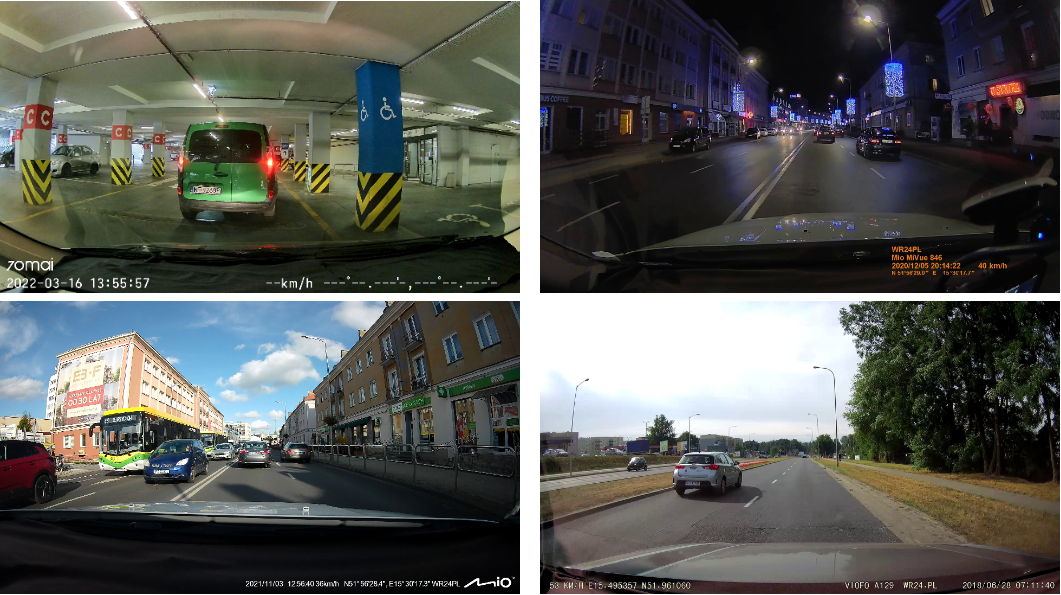
\includegraphics[scale=0.4]{Pictures/captured_frames}
    \caption{Pozyskane zdjęcia z wideorejestratora (źródło: opracowanie własne).}
    \label{fig:captured_frame}
\end{figure}
\FloatBarrier

Kolejnym krokiem niezbędnym przed rozpoczęciem procesu uczenia było nadanie etykiet obiektom na wyeksportowanych zdjęciach.
W tym celu opracowano skrypt służący do ręcznego oznaczania tablic rejestracyjnych.
Skrypt powstał na podstawie narzędzia~\cite{haar_object_marker}.
Jego fragment w postaci pseudokodu przedstawiono na poniższym schemacie.
\begin{algorithm}
    \caption{Procedura zapisująca współrzędne pozytywnych próbek.}
    \begin{algorithmic}[1]
        \label{create_positives}
        \Procedure{ObjectMarkerOnClick}{$(event, x, y)$}
            \If{$event == $ kliknięcie lewego przycisku myszy}
                \If {Liczba kliknięć jest nieparzysta}
                    \State Przypisz współrzędne $(x,y)$ kliknięcia jako początek obszaru próbki.
                \Else
                    \State Przypisz współrzędne $(x,y)$ kliknięcia jako koniec obszaru próbki.
                    \State Zwiększ liczbę obiektów w obrazie.
                    \State Przeskaluj współrzędne do stałej wartości.
                    \State Dodaj do listy pozytywów zaznaczony fragment.
                \EndIf
            \EndIf
        \EndProcedure
    \end{algorithmic}
\end{algorithm}
\FloatBarrier


%\begin{lstlisting}[language=Python, caption=Funkcja do oznaczania fragmentów obrazu zawierających poszukiwany obiekt., label=alg:positive_creator]
%import cv2
%
%def obj_marker(event, x, y):
%    global click_count
%    global debug
%    global obj_list
%    global obj_count
%    global frameName
%    global x1
%    global y1
%    global w
%    global h
%    global frame
%    global frameResized
%    if event == cv2.EVENT_LBUTTONDOWN:
%        click_count += 1
%        if click_count % 2 == 1:
%            x1 = x
%            y1 = y
%        else:
%            orgShape = frame.shape
%            ratioH = orgShape[0] / 1080
%            ratioW = orgShape[1] / 1920
%
%            w = abs(x1 - x)
%            h = abs(y1 - y)
%            obj_count += 1
%            if x1 > x:
%                x1 = x
%            if y1 > y:
%                y1 = y
%            obj_list.append('%d %d %d %d ' % (x1 * ratioW, y1 * ratioH, w * ratioW, h * ratioH))
%            cv2.rectangle(frameResized, (x1, y1), (x1 + w, y1 + h), (0, 255, 0), 1)
%            cv2.imshow(frameName, frameResized)
%\end{lstlisting}
Wszystkie zdjęcia wyświetlano po kolei na ekranie.
Zdarzenie kliknięcia myszką na obrazie przechwytywano w programie.
Pierwsze kliknięcie oznaczało współrzędne początku obszaru pozytywnej próbki.
Drugie kliknięcie oznaczało współrzędne końca rozpatrywanego obszaru.
Jak wspomniano wcześniej, obrazy posiadały różne rozdzielczości, często przewyższające rozdzielczość monitora.
Aby zdjęcia wyświetlały się poprawnie, skalowano je do rozdzielczości ekranu, na którym przeprowadzono operację nadawania etykiet.
Pozyskane koordynaty zapisywano do globalnej tablicy.
Na koniec procesu dane zapisano do pliku tekstowego, z którego odczytywano dane podczas etapu uczenia.
Dane w pliku zapisano w formacie \textit{ścieżka do pliku, liczba obiektów w pliku, kolejno współrzędne każdego z prostokątów}.
W tabeli~\ref{tab:tab_data_set_characteristics} przedstawiono cechy charakterystyczne przygotowanego zbioru.
\begin{table}[h]
    \centering
    \caption{Parametry opracowanego zbioru.}
    \begin{tabular}{l l l}
        \toprule
        \textbf{Parametr}                      & \textbf{Wartość}                                     \\
        \midrule
        Liczba zdjęć                           & 10985                                                \\
        Format zdjęć                           & JPG                                                  \\
        Liczba zdjęć zawierających tablice     & 5248                                                 \\
        Ogółem liczba tablic                   & 10301                                                \\
        Zakres liczby tablic na jednym zdjęciu & 0--6                                                 \\
        Średnia wysokość próbki                & 38px                                                 \\
        Średnia szerokość próbki               & 91px                                                 \\
        Maksymalne rozmiary próbki             & 378$\times$136px                                     \\
        Minimalne rozmiary próbki              & 15$\times$11px                                       \\
        Rozdzielczości zdjęć                   & 1920$\times$1080, 2560$\times$1440, 3840$\times$2160 \\
        Liczba klatek na sekundę               & 30 kl/s, 60 kl/s                                     \\
        \bottomrule
    \end{tabular}
    \label{tab:tab_data_set_characteristics}
\end{table}